\documentclass[PianoDiProgetto.tex]{subfiles}

\begin{document}

\chapter{Modello di sviluppo}
Come modello di sviluppo per il ciclo di vita del software è stato deciso di adottare il \textbf{modello incrementale}, per garantire qualità, conformità e maturità del prodotto.

\section{Modello incrementale}
In un modello di sviluppo incrementale, inizialmente viene pianificato il numero di incrementi da eseguire e il cliente identifica i requisiti fondamentali e quelli desiderabili del prodotto software. A ciascuno di questi viene poi associata una priorità. I requisiti da sviluppare vengono poi suddivisi nei vari incrementi, mettendo nei primi quelli con priorità maggiore. La consegna del prodotto quindi non viene eseguita tutta insieme, ma è anch'essa incrementale.\\
Durante la fase di sviluppo di un incremento non è possibile modificare i requisiti decisi prima di iniziare lo sviluppo dell'incremento corrente, ma è invece accettabile aggiungere dei requisiti da sviluppare negli incrementi successivi. Al termine dello sviluppo, l'incremento viene aggiunto al prodotto software, dimostrandone il grado di efficacia. Se il prodotto non è finito, si procederà poi con gli incrementi successivi. I \textbf{vantaggi} principali di questo modello sono:
\begin{itemize}
	\item sviluppando inizialmente i requisiti di maggiore importanza e priorità, essi saranno soggetti a maggiori verifiche;
	\item producendo rilasci continui è possibile sin dal primo avere un prototipo del prodotto.
\end{itemize}

\begin{figure}[h] %TODO usare \nImg e non far andare a pagina nuova immagine
	\centering
	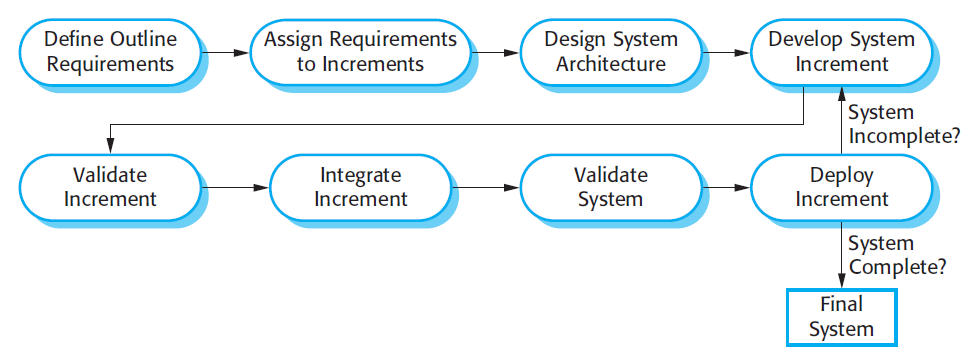
\includegraphics[width=10cm]{images/modIncrementale.png}
	\label{fig:foo}
	\caption{Modello incrementale}
\end{figure} 
\end{document}